
\documentclass[12pt]{article}
\usepackage{geometry} % see geometry.pdf on how to lay out the page. There's lots.
\usepackage{graphicx}
\usepackage{graphics}
\usepackage{natbib}
\usepackage{amsmath}
\usepackage{listings}
\usepackage{url}
\usepackage{needspace}
\usepackage{booktabs}
\usepackage{topcapt}
%\geometry{a4paper} % or letter or a5paper or ... etc
% \geometry{landscape} % rotated page geometry

\newcommand{\code}[1]{{\tt #1}}


% See the ``Article customise'' template for come common customisations

\title{The ModelGrid Package}
\author{Greg Tucker}
\date{Last update May 2014} % delete this line to display the current date

%%% BEGIN DOCUMENT
\begin{document}

\lstset{ %
language=Python,                % choose language
%basicstyle=\footnotesize,       % size of fonts used for code
numbers=left,                   % where to put line-numbers
numberstyle=\footnotesize,      % size used for line-numbers
stepnumber=1,                   % the step between two line-numbers. If it is 1 each line will be numbered
numbersep=5pt,                  % how far the line-numbers are from the code
%backgroundcolor=\color{white},  % choose the background color. You must add \usepackage{color}
showspaces=false,               % show spaces adding particular underscores
showstringspaces=false,         % underline spaces within strings
showtabs=false,                 % show tabs within strings adding particular underscores
frame=single,           % adds a frame around the code
tabsize=2,          % sets default tabsize to 2 spaces
captionpos=t,           % sets the caption-position to bottom
breaklines=true,        % sets automatic line breaking
breakatwhitespace=false,    % sets if automatic breaks should only happen at whitespace
columns=fullflexible,
basicstyle=\footnotesize\ttfamily,
escapeinside={\%*}{*)}          % if you want to add a comment within your code
}

\maketitle
%\tableofcontents

\section{Overview}

ModelGrid is an open-source software package that creates and manages a regular or irregular grid for building 2D numerical simulation models. ModelGrid is especially useful for finite-volume (FV) and finite-difference (FD) models, but also can be used for a variety of other applications. ModelGrid provides efficient built-in functions for common operations in FD and FV models, such as calculating local gradients and integrating fluxes around the perimeter of grid cells. Staggered-grid models are especially easy to implement with ModelGrid.
A novel feature of ModelGrid is the ability to switch seamlessly between structured and unstructured grids.

This document provides a basic introduction to building applications using ModelGrid. It covers: (1) how grids are represented, (2) a tutorial example in building a diffusion-model application, and (3) a guide to ModelGrid's methods and data structures. ModelGrid is written in python. It is a component of the Landlab modeling package.

\subsection{How a Grid is Represented}

%%%%%%%%%%% FIGURE %%%%%%%%%%%
 \begin{figure}[h!]
    \centering
    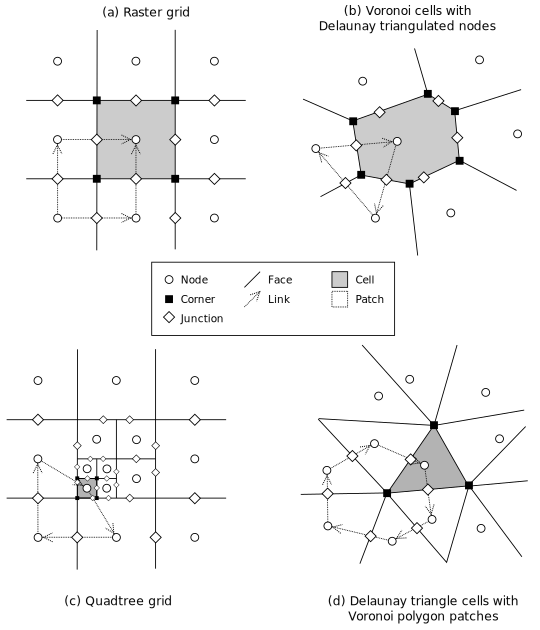
\includegraphics[scale=0.92]{grid_schematic.pdf}
    \caption{Elements of a model grid. Each grid comprises nodes, cells, faces, corners, patches, links, directed edges, and junctions. (Note that not all links, edges, and patches are shown, and only one representative cell is shaded.)}
   \label{grid}
\end{figure}
%%%%%%%%%%%%%%%%%%%%%%%%%%%

Figure~\ref{grid} illustrates how ModelGrid represents a simulation grid. The grid contains a set of $(x,y)$ points called {\em nodes}. In a typical finite-difference model, nodes are the locations at which one tracks scalar state variables, such as water depth, land elevation, or temperature. Each node is associated with a polygon called a {\em cell}. Each cell is bounded by a set of line segments known as {\em faces}, which it shares with its neighboring cells.

In the simple case of a regular (raster) grid, the cells are square, the nodes are the center points of the cells (Figure~\ref{grid}a), and the faces have identical length (equal to the node spacing). In a Voronoi-Delaunay grid, the cells are Voronoi polygons (also known as Theissen polygons) (Figure~\ref{grid}b). In this case, each cell represents the surface area that is closer to its own node than to any other node in the grid. The faces then represent locations that are equidistant between two adjacent nodes. Other grid configurations are possible as well. For examples, cells could be square elements in a quad-tree grid (Figure~\ref{grid}c), or triangular elements with nodes at their circumcenters (Figure~\ref{grid}d).

Each pair of adjacent cells is connected by a line segment called a {\em link} (Figure~\ref{grid}, dashed line). Each link connects a {\em from node} and a {to node}, so it has direction as well as position and length. In some cases, it may be useful to have each pair of adjacent cells connected by two vectors: one pointing one way, and a second pointing the opposite way \citep{guibas1985primitives,tucker2001object}. These vectors are known as {\em directed edges} (Figure~\ref{grid}, gray arrows). 

Finite-difference and finite-volume models usually need to calculate spatial gradients in one or more scalar variables, and often these gradients are evaluated between pairs of adjacent nodes. ModelGrid makes these calculations easier for programmers by providing built-in functions to calculate gradients along links, and allowing applications to associate an array of gradient values with their corresponding links or edges.

The cell vertices are called {\em corners} (Figure~\ref{grid}, solid squares). Each face is therefore a line segment connecting two corners. The intersection of a face and a link (or directed edge) is known as a {\em junction} (Figure~\ref{grid}, open diamonds). Often, it is useful to calculate scalar values (say, ice thickness in a glacier) at nodes, and vector values (say, ice velocity) at junctions. This approach is sometimes referred to as a staggered-grid scheme. It lends itself naturally to finite-volume methods, in which one computes fluxes of mass, momentum, or energy across cell faces, and maintains conservation of mass within cells \citep[e.g.,][]{versteeg2007introduction}.

Notice that the links also enclose a set of polygons that are offset from the cells. These secondary polygons are known as {\em patches} (Figure~\ref{grid}, dotted). This means that any grid comprises two complementary tesselations: one made of cells, and one made of patches. If one of these is a Voronoi tessellation, the other is a Delaunay triangulation. For this reason, Delaunay triangulations and Voronoi diagrams are said to be dual to one another: for any given Delaunay triangulation, there is a unique corresponding Voronoi diagram \citep[e.g.,][]{braun1997modelling,tucker2001object}. With ModelGrid, one can create a mesh with either Voronoi polygons or Delaunay triangles as cells (Figure~\ref{grid}, b and d). Alternatively, with a raster grid, one simply has two sets of square elements that are offset by half the grid spacing (Figure~\ref{grid}a). Whatever the form of the tessellation, ModelGrid keeps track of the geometry and topology of the grid. For example, one can call various ModelGrid functions to obtain lists of the $(x,y)$ coordinates of nodes, corners, and junctions; get lists of neighbors for any cell; get the endpoints of any link or directed edge, and so on. These functions are listed and described below. 

\subsection{How Boundaries are Managed}

An important component of any numerical model is the method for handling boundary conditions. In general, it's up to the application developer to manage boundary conditions for each variable. However, ModelGrid makes this task a bit easier by providing lists of nodes and links that lie along the boundary of the grid, and those that lie in the interior. It also allows you to ``de-activate'' portions of the grid perimeter, so that they effectively act as walls.

Let's look first at how ModelGrid treats its own geometrical boundaries. The outermost elements of a grid are nodes and links (as opposed to corners and faces). For example, Figure~\ref{raster4x5} shows a sketch of a regular four-row by five-column grid created by RasterModelGrid. The edges of the grid are composed of nodes and links. Only the inner six nodes have cells around them; the remaining 14 nodes form the perimeter of the grid.

All nodes are tagged as either {\em boundary} or {\em interior}. Those on the perimeter of the grid are automatically tagged as boundary nodes. Nodes on the inside are {\em interior} by default, but it is possible to tag some of them as {\em boundary} instead (this would be useful, for example, if you wanted to represent an irregular region inside a regular grid). In the example shown in Figure~\ref{raster4x5}, all the inner nodes are {\em active interior}, and all perimeter nodes are {\em active boundary}. 

Boundary nodes are flagged as either {\em open (active)} or {\em closed (inactive),} all links are tagged as active or inactive. An {\em active link} is one that joins either two interior nodes, or an  
{\em interior} and an {\em open boundary} node (Figure~\ref{raster4x5openclosed}). You can use this distinction in models to implement closed boundaries by performing flow calculations only on active links, as the following simple example illustrates.


%%%%%%%%%%% FIGURE %%%%%%%%%%%
 \begin{figure}[h!]
    \centering
    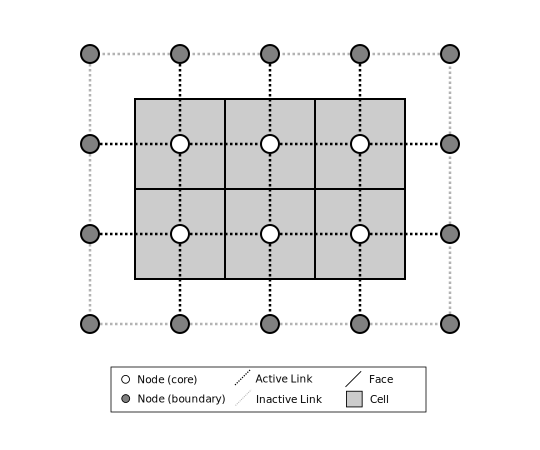
\includegraphics{example_raster_grid.pdf}
    \caption{Illustration of a simple four-row by five-column raster grid created with RasterModelGrid. By default, all perimeter nodes are tagged as active (fixed value) boundaries, and all interior cells are tagged as active interior. An active link is one that connects either two active interior cells, or one active interior and one active boundary.}
   \label{raster4x5}
\end{figure}
%%%%%%%%%%%%%%%%%%%%%%%%%%%

%%%%%%%%%%% FIGURE %%%%%%%%%%%
 \begin{figure}[h!]
    \centering
    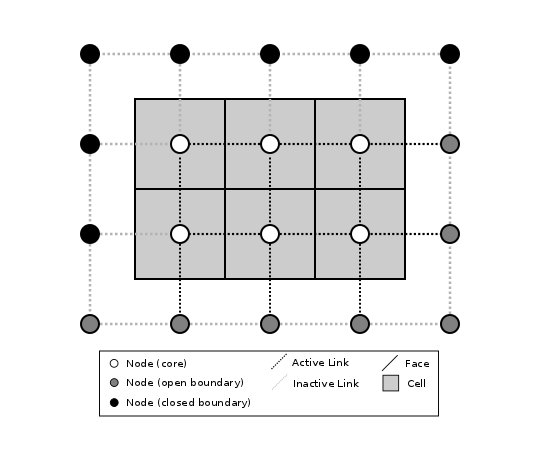
\includegraphics{example_raster_grid_with_closed_boundaries.pdf}
    \caption{Illustration of a simple four-row by five-column raster grid with a combination of open and closed boundaries.}
   \label{raster4x5openclosed}
\end{figure}
%%%%%%%%%%%%%%%%%%%%%%%%%%%



%In ModelGrid, the boundaries of the grid are treated by assigning a {\em boundary code} to each node. The boundary codes are:
%\begin{itemize}
%\item \verb|INTERIOR_NODE|: node is a normal, active interior node.
%\item \verb|FIXED_VALUE_BOUNDARY = 1|: node is meant to have a prescribed value, set by the application. For example, one might maintain a constant elevation, temperature, or ice thickness here.
%\item \verb|FIXED_GRADIENT_BOUNDARY = 2|: indicates that a prescribed gradient is meant to exist between the node and any adjacent interior nodes.
%\item \verb|TRACKS_CELL_BOUNDARY = 3|: indicates that the value at the node is meant to mirror that at another node.
%\item \verb|INACTIVE_BOUNDARY = 4|: indicates that the node is ``inactive,'' meaning that it should not give or receive any flow.
%\end{itemize}
%For the most part, these codes are provided for the convenience of the application developer. The key distinction that ModelGrid actually uses


\section{ModelGrid Example: Diffusion} 

The following is a simple tutorial in which we use ModelGrid to build an explicit, staggered-grid model of diffusion. The mathematics of diffusion describe quite a few different phenomena, among them heat conduction in solids, chemical diffusion of dissolved material, transport of momentum in a viscous shear flow, and transport of soil on hillslopes. To make this exercise concrete, we will use the latter as our working example, though in fact the solution could apply to any of these systems.

To work through this example, you can type in and run the code below, or find a copy at \url{http://csdms.colorado.edu/trac/landlab/} or \url{http://csdms.colorado.edu/wiki/Model:LandLab}. The complete source code for the diffusion model is listed below. Line numbers are included to make it easier to refer to particular lines of code (of course, these numbers are not part of the source code). After the listing, we will take a closer look at each piece of the code in turn. Output from the the diffusion model is shown in Figure~\ref{basicdiffmod}.

%%%%%%%%%%% FIGURE %%%%%%%%%%%
 \begin{figure}[h!]
    \centering
    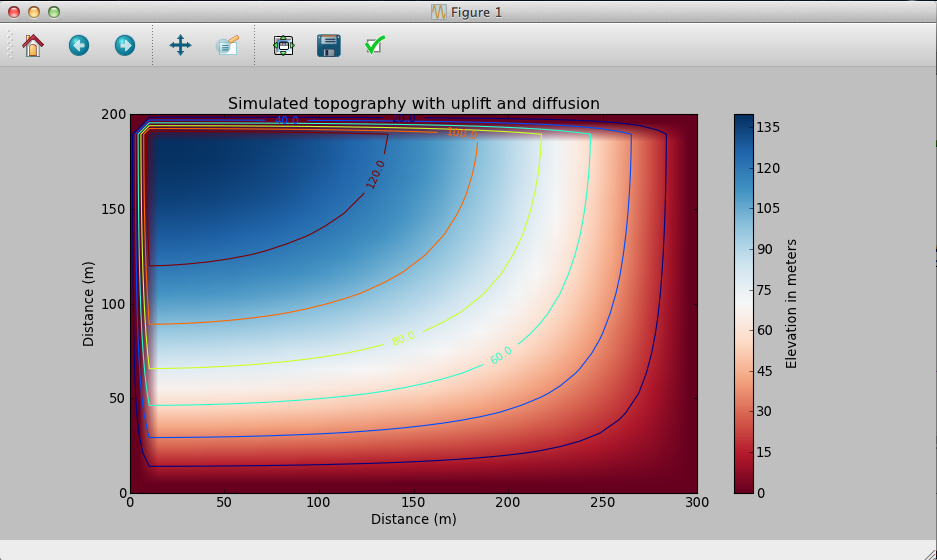
\includegraphics[scale=0.45]{basic_diffusion_example.png}
    \caption{Output from \code{diffusion\_with\_model\_grid.py}.}
   \label{basicdiffmod}
\end{figure}
%%%%%%%%%%%%%%%%%%%%%%%%%%%



\lstinputlisting[language=Python,caption={diffusion\_with\_model\_grid.py}]{diffusion_with_model_grid.py}


\newpage
\subsection{Importing Packages}

\lstinputlisting[firstnumber=11,firstline=11,lastline=12]{diffusion_with_model_grid.py}

We start by importing the grid class {\tt RasterModelGrid} from the {\tt landlab} package (note that the {\tt landlab} package must first be installed; see instructions at \url{http://csdms.colorado.edu/trac/landlab/}). We'll also import {\tt pylab} so we can plot the results, and {\tt time} so we can report the time it takes to run the model.


\subsection{Setting the User-Defined Parameters}

\lstinputlisting[firstnumber=14,firstline=14,lastline=29]{diffusion_with_model_grid.py}

The first thing we'll do is set a group of user-defined parameters. The size of the grid is set by \code{numrows} and \code{numcols}, with cell spacing \code{dx}. In this example, we have a 20 by 30 grid with 10~m grid spacing, so our domain represents a 200 by 300~m rectangular patch of land. The diffusivity coefficient \code{kd} describes the efficiency of soil creep, while the \code{uplift\_rate} indicates how fast the land is rising relative to base level along its boundaries. Finally, we set how many time steps we want to compute.

Note that the code for our simple program lives inside a \code{main()} function. This isn't strictly necessary---we could have put the code in the file without a \code{main()} function and it would work just fine when we run it---but it is good Python practice, and will be helpful later on.

\break
\subsection{Calculating Derived Parameters}

\lstinputlisting[firstnumber=31,firstline=31,lastline=33]{diffusion_with_model_grid.py}

Next, we calculate the values of parameters that are derived from the user-defined parameters. In this case, we have just one: the time-step size, which is set by the Courant-Friedrichs-Lewy condition for an explicit, finite-difference solution to the diffusion equation (to be on the safe side, we multiply the ratio $\Delta x^2 / k_d$ by 0.1 instead of the theoretical limit of 1/2). With the parameter values above, $\Delta t = 1000$ years, so our total run duration will be one million years. Remember, though, that the same code could be used for any diffusion application with a source term. For instance, we could model conductive heat flow, with $k_d$ representing thermal diffusivity and \code{uplift\_rate} representing steady head input.


\subsection{Creating and Configuring the Grid}

\lstinputlisting[firstnumber=34,firstline=34,lastline=38]{diffusion_with_model_grid.py}

Our model grid is created with a call to \code{RasterModelGrid()}, which returns a raster model grid object with the given dimensions and node spacing. %We then set up this grid with a call to its \code{initialize} method, passing it the desired grid dimensions and spacing.

For our boundary conditions, we would like to keep the nodes along the bottom and right edges of the grid fixed at zero elevation. We also want to have the top and left boundaries represent ridge-lines with a fixed horizontal position and no flow of sediment in or out. To accomplish this, we call the \code{set\_inactive\_boundaries} method on line 38. The method takes four boolean arguments, which indicate whether there should be closed boundary condition on the top, right, bottom, and left sides of the grid. Here we have set the flag to \code{True} for the top and left sides. This means that the links connecting the interior nodes to the perimeter nodes along these two sides will be flagged as inactive, just as illustrated (with a smaller grid) in Figure~\ref{raster4x5openclosed}. As we'll see in a moment, we will simply not bother to calculate any mass flux across these closed boundaries.


\subsection{Creating Data}

\lstinputlisting[firstnumber=40,firstline=40,lastline=50]{diffusion_with_model_grid.py}

Our state variable, $z(x,y,t)$, represents the land surface elevation. One of the unique aspects of ModelGrid is that grid-based variables like $z$ are represented as 1D rather than 2D Numpy arrays. Why do it this way, if we have a regular grid that naturally lends itself to 2D arrays? The answer is that we might want to have an irregular, unstructured grid, which is much easier to handle with 1D arrays of values. By using 1D arrays for all types of ModelGrid, we allow the user to switch seamlessly between structured and unstructured grids.

We create our data structure for $z$ values with  \code{add\_zeros}, a ModelGrid method that creates and returns a 1D Numpy array filled with zeros (behind the scenes, it also ``attaches'' the array to the grid; we'll see later why this is useful). The length of the array is equal to the number of nodes in the grid ($20\times 30=600$), which makes sense because we want to have an elevation value associated with every node in the grid.

When we update elevation values, we will want to operate only on the active cells. To help with this, we call the \code{get\_active\_cell\_node\_ids} method. This method returns a 1D numpy array of integers that represent the node ID numbers associated with all of the active cells (of which there are $18\times 28 = 504$). Finally, we display a message to tell the user that we're about to run and with what time step size.


\subsection{Main Loop}

Our model implements a finite-volume solution to the diffusion equation. The idea here is that we calculate sediment fluxes around the perimeter of each cell. We then integrate these fluxes forward in time to calculate the net change in volume, which is divided by the cell's surface area to obtain an equivalent change in height. The numerical solution is given by:
\begin{equation}
\frac{d z_i}{dt} \approx \frac{z^{T+1}_i-z^T_i}{\Delta t}
= - \frac{1}{\Lambda_i} \sum_{j=1}^{N_i} \mathbf{q}_{Sij}^T \lambda_{ij}.
\label{eq:dzdt}
\end{equation}
Here, $z_i^T$ is the elevation at node $i$ at time step $T$, $t$ is time, $\Lambda_i$ is the surface area of cell $i$, $N_i$ is the number of cells adjacent to $i$ (called the cell's {\em neighbors}), $\mathbf{q}_{Sij}^T$ is the sediment flux per unit face width from cell $i$ to cell $j$, and $\lambda_{ij}$ is the width of the face between cells $i$ and $j$. The flux between a pair of adjacent cells is the product of the slope (positive upward) between their associated nodes, $\mathbf{S}_{ij}$, and a transport coefficient, $k_d$,
\begin{equation}
\mathbf{q}_{Sij} = - k_d \mathbf{S}_{ij} = - k_d \frac{z_j-z_i}{L_{ij}}
\end{equation}
where $L_{ij}$ is the length of the link connecting nodes $i$ and $j$. Notice that elevation values (which are scalars) are associated with nodes, while slopes and sediment fluxes (which are vectors) are associated with links and faces. If we want to think of the slopes and fluxes as being calculated at a particular point, that point is the junction between a link and its corresponding face (Figure~\ref{grid}).

Because we are using a regular (raster) grid with node spacing $\Delta x$, the face width and link length are both equal to $\Delta x$ everywhere, and the cell area $\Lambda=\Delta x^2$. This would not be true, however, for an unstructured grid.

\subsection{Calculating gradients and sediment fluxes}

\lstinputlisting[firstnumber=53,firstline=53,lastline=59]{diffusion_with_model_grid.py}

In order to calculate new elevation values, the first quantity we need to know is the gradient (slope) values between all the node pairs. We can calculate this in a single line of code using ModelGrid's \code{calculate\_gradients\_at\_active\_links} method. This method takes a single argument: a 1D numpy array of scalar values associated with nodes. The length of this array must be the same as the number of nodes in the grid. The method calculates the gradients in \code{z} between each pair of nodes. It returns a 1D numpy array, \code{g} (for gradient), the size of which is the same as the number of active links in the grid (the difference between active and inactive links is illustrated Figures~\ref{raster4x5} and \ref{raster4x5openclosed}). The sign of each value of \code{g} is positive when the slope runs uphill from a link's {\em from node} to its {\em to node}, and negative otherwise.

To calculate the sediment fluxes, we multiply each gradient value by the transport coefficient \code{kd}. The minus sign simply means that the sediment goes downhill: where the gradient is negative, the flux should be positive, and vice versa. Here, we are taking advantage of numpy's ability to perform mathematical operations on entire arrays in a single line of code, rather than having to write out a \code{for} loop. Line 60 in our code multiplies \code{ks} by every value of \code{g}, and returns the result as a numpy array the same size as \code{g}.

\subsection{Calculating net fluxes in and out of cells}

\lstinputlisting[firstnumber=60,firstline=60,lastline=61]{diffusion_with_model_grid.py}

Now that we know the unit flux associated with each link and its corresponding cell face, the next thing we need to do is add up the total flux around the perimeter of each cell. In other words, we need to calculate the summation in equation (\ref{eq:dzdt}). ModelGrid allows us to do this in one line of code, by calling the \code{calculate\_flux\_divergence\_at\_nodes} method. This method takes a single argument: a 1D Numpy array containing the flux per unit width at each face in the grid. The method multiplies each unit flux by its corresponding face width, adds up the fluxes across each face for each cell, and divides the result by the surface area of the cell. It returns a 1D Numpy array that contains the net rate of change of volume per unit cell area. The length of this array is the same as the number of nodes in the grid. We will store the result in \code{dqsds}.

If the boundary nodes around the grid perimeter do not have associated cells, why do we bother calculating net fluxes for them? In fact, we do not need to; we could have called the method \code{calculate\_flux\_divergence\_at\_active\_cells} instead. This would have given us an array the length of the number of active cells, not nodes. There are two reasons to do the net flux calculation at all nodes. The first is simply that the node-based method is slightly faster than the cell-based version. The second is that by using nodes, we retain some information about the flow of mass into the boundary cells. This could be useful in testing whether our model correctly balances mass (though we do not actually use that capability in this example).

\newpage
\subsection{Updating elevations}

\lstinputlisting[firstnumber=63,firstline=63,lastline=67]{diffusion_with_model_grid.py}

When we calculated flux divergence, we got back an array of numbers, \code{dqsds}, that represents the deposition (positive) or erosion (negative) rate of each cell. Now we need to combine this with the source term---representing rock uplift relative to the base level at the model's fixed boundaries---in order to calculate the total rate of elevation change at the nodes. Once we've calculated rates of change, we update all node elevations by simply multiplying \code{dzdt} by our time step size. We do not want to change the elevations of the boundary nodes, however, and so we perform the update only on the interior cells. Because we are using numpy arrays, we can isolate the interior cells simply by putting our array of node IDs for interior cells inside square brackets. 

%\subsection{Updating no-flux boundaries}
%
%\lstinputlisting[firstnumber=72,firstline=72,lastline=73]{diffusion_with_model_grid.py}
%
%The last step in the loop is to update any zero-gradient (no-flux) boundaries. The call to \code{update\_noflux\_boundaries} simply sets the elevation of any no-flux boundary nodes to the elevation of the adjacent interior neighbor. This way, the gradient and hence the flux will be zero at that interface.


\subsection{Plotting the Result}

\lstinputlisting[firstnumber=72,firstline=72,lastline=92]{diffusion_with_model_grid.py}

The last section of the \code{main} function plots the result of our calculation. We do this using pylab's \code{imshow} and \code{contour} functions to create a colored image of topography overlain by contours. To use these functions, we need our elevations to be ordered in a 2D array. We obtain a 2D array version of our \code{z} values through a call to RasterModelGrid's \code{node\_vector\_to\_raster} method.

%\newpage
\subsection{Running the \code{main()} function}

\lstinputlisting[firstnumber=95,firstline=95,lastline=96]{diffusion_with_model_grid.py}

The last two lines of code are standard Python syntax. They will execute the \code{main} function when the code is run, but not when the code is simply imported as a module.

That's it. The 2D diffusion code is less than 100 lines long. In fact, only about 20 of these actually implement the diffusion calculation; the rest handle plotting, comments, blank lines, etc.

\subsection{Checking against the analytical solution}

To test the diffusion model against an analytical solution, we can change the setup to have closed boundaries on two opposite sides, by modifying line 39 to read:

\code{mg.set\_inactive\_boundaries(True, False, True, False)}

This change makes the solution symmetrical in the $y$ direction, so that we can compare it with a 1D analytical solution. For a 1D steady state configuration with a constant source term (baselevel lowering) and two fixed boundaries, the elevation field is a parabola:
\begin{equation}
z(x') = \frac{U}{2K_d} \left( L^2 - x'^2 \right),
\end{equation}
where $L$ is the half-length of the domain and $x'$ is a transformed $x$ coordinate such that $x'=0$ at the ridge crest. The numerical solution fits the analytical solution quite well (Figure~\ref{diffrasteranalytical}).

%%%%%%%%%%% FIGURE %%%%%%%%%%%
 \begin{figure}[h!]
    \centering
    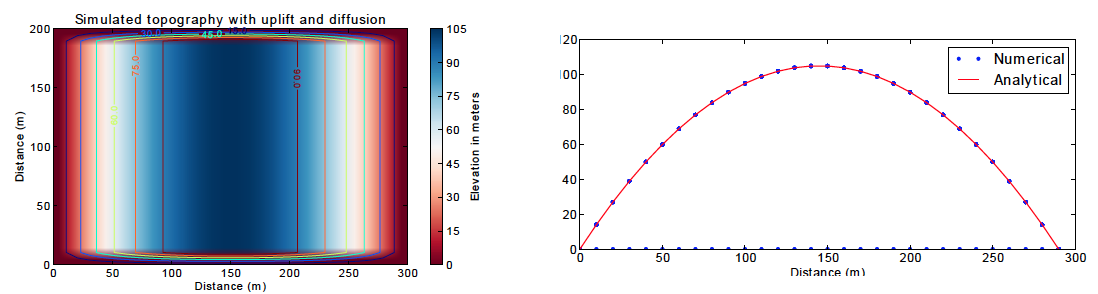
\includegraphics{diffusion_raster_with_analytical.pdf}
    \caption{Diffusion model with two opposite sides as open boundaries. Left: overhead view. Right: side view showing nodes (blue dots) and 1D analytical solution (red line).}
   \label{diffrasteranalytical}
\end{figure}
%%%%%%%%%%%%%%%%%%%%%%%%%%%


%%%%%%%%

\section{Example 2: Overland Flow}

In this second example, we look at an implementation of the storage-cell algorithm of \citet{bates2010simple} for modeling flood inundation. In this example, we will use a flat terrain, and prescribe a water depth of 2.5 meters at the left side of the grid. This will create a wave that travels from left to right across the grid. The output is shown in Figure~\ref{inundation}.

%%%%%%%%%%% FIGURE %%%%%%%%%%%
 \begin{figure}[h!]
    \centering
    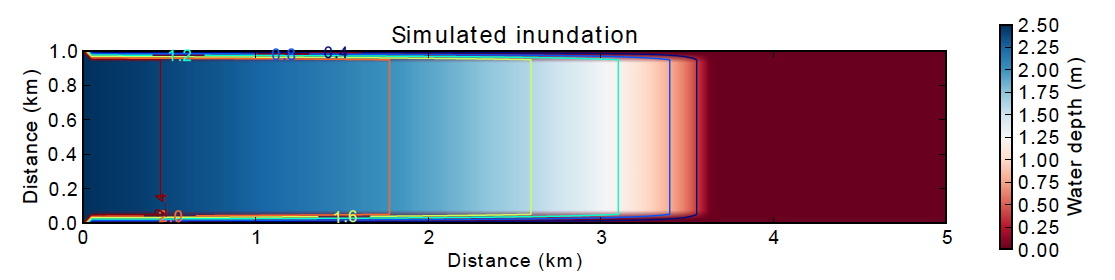
\includegraphics{inundation.pdf}
    \caption{Simulated flood-wave propagation.}
   \label{inundation}
\end{figure}
%%%%%%%%%%%%%%%%%%%%%%%%%%%

\subsection{Overland Flow Code Listing}

The source code can be found in \code{overland\_flow\_with\_model\_grid.py}.

\lstinputlisting[firstnumber=1,firstline=1,lastline=143]{overland_flow_with_model_grid.py}

\subsection{Packages}

\lstinputlisting[firstnumber=11,firstline=11,lastline=13]{overland_flow_with_model_grid.py}

For this program, we'll need ModelGrid as well as the pylab, time, and numpy packages.

\subsection{User-Defined Parameters}

\lstinputlisting[firstnumber=24,firstline=24,lastline=33]{overland_flow_with_model_grid.py}

Several of the user-defined parameters are the same as those used in the diffusion example: the dimensions and cell size of our raster grid, and the duration of the run. Here the duration is in seconds. In addition, we need to specify the Manning roughness coefficient (\code{n}), the initial water depth (here set to 1 mm), the water depth along the left-hand boundary, gravitational acceleration, and a time-step factor.

\subsection{Derived Parameters}

\lstinputlisting[firstnumber=35,firstline=35,lastline=39]{overland_flow_with_model_grid.py}

Here, we pre-calculate the value of 10/3 so as to avoid repeating a division operation throughout the main loop. We also set up some variables to track the progress of the run. The elapsed time refers here to model time. In this model, we use a variable time-step size, and so rather than counting through a predetermined number of iterations, we instead keep track of the elapsed run time and halt the simulation when we reach the desired run duration.

The \code{report\_interval} refers to clock time rather than run time. Every two seconds of clock time, we will report the percentage completion to the user, so that he/she is aware that the run is progressing and has an idea how much more is left to go. The variable \code{next\_report} keeps track of the next time (on the clock) to report progress to the user.

\newpage
\subsection{Setting up the grid and state variables}

\lstinputlisting[firstnumber=41,firstline=41,lastline=60]{overland_flow_with_model_grid.py}

Next, we create and configure a raster grid. In this example, we'll have the left and right boundaries open and the top and bottom closed; we set this up with a call to \code{set\_inactive\_boundaries} on line 47.

Our key variables are as follows: land elevation, \code{z} (which remains constant and uniform at zero in this example), water depth, \code{h} (which starts out at \code{h\_init}), discharge per unit width, \code{q}, and the rate of change of water depth, \code{dhdt}. Three of these---elevation, depth, and $dh/dt$, are scalars that are evaluated at nodes. The fourth, discharge, is evaluated at active links.

In this example, we will have the left boundary maintain a fixed water depth of 2.5 m. To accomplish this, we first obtain a list of the ID numbers of the boundary nodes that lie along the left grid edge by calling RasterModelGrid's \code{left\_edge\_node\_ids()} method, which returns a Numpy array containing the IDs. We then use them to set the new depth values on the following line. Finally, on line 60, we obtain a list of interior node IDs, just as we did in the diffusion example.

\subsection{Main loop, part 1}

\lstinputlisting[firstnumber=68,firstline=68,lastline=93]{overland_flow_with_model_grid.py}

The main loop uses a \code{while} rather than a \code{for} loop because the time-step size is variable. We begin with a block of code that prints the percentage completion to the screen every two seconds. After this, we calculate a maximum time-step size size using the formula of \citet{bates2010simple}, which depends on grid-cell spacing and on the shallow water wave celerity, $\sqrt{g h}$. For water depth, we use the maximum value in the grid, because it is this value that will have the greatest celerity and therefore be most restrictive.

The next several lines calculate unit discharge values along each active link. To do this, we need to know the effective water depth at each of these locations. \citet{bates2010simple} recommend using the difference between the highest water-surface elevation and the highest bed-surface elevation at each pair of adjacent nodes---that is, at each active link. To find these maximum values, we call the \code{active\_link\_max} function, first with bed elevation, and then with water-surface elevation, \code{w}. The resulting effective flow depths at the active links are stored in Numpy array called \code{hflow}. 

Calculating discharge also requires us to know the water-surface gradient at each active link. We find this by calling \code{calculate\_gradients\_at\_active\_links} and passing it the water-surface height. We then have everything we need to calculate the discharge values using the \citet{bates2010simple} formula, which is done on lines 92 and 93.

\subsection{Main loop, part 2}

\lstinputlisting[firstnumber=95,firstline=95,lastline=113]{overland_flow_with_model_grid.py}

Because we have no source term in the flow equations---we are assuming there is no rainfall or infiltration to add or remove water in each cell---the rate of depth change is equal to $-\nabla q$, the divergence of water discharge. Just as in the diffusion example, we can calculate the flux divergence in a single line with help from the \code{calculate\_flux\_divergence\_at\_nodes} method.

The next block of code provides a second limit on time-step size, designed to prevent water depth from becoming negative. At some locations in the grid, it is possible that the rate of change of water depth will be negative, meaning that the water depth is becoming shallower over time. If we were to extrapolate this shallowing too far into the future, by taking too big a time step, we could end up with negative water depth. To avoid this situation, we first determine whether there are any locations where \code{dhdt} is negative, using the Numpy \code{amin} function. If there are, we call the Numpy \code{where} function to obtain a list of the node IDs at which the water depth is shallowing. The next line calculates the time it would take to reach zero water thickness. On line 104, we find the minimum of these time intervals, and multiply it by the \code{alpha} time-step parameter. This ensures that we won't actually completely drain any cells of water. Finally, we determine which limiting time-step is smaller: \code{dtmax}, which reflects the limitation due to fluid velocity, or \code{dtmax2}, which is the limitation due to cell drainage. If no cells have $dh/dt<0$, then we simply use the fluid-velocity time step size.

Line 110 updates the values of water depth at all interior cells. Finally, line 113 increments the total elapsed time.

\subsection{Plotting the results}

\lstinputlisting[firstnumber=118,firstline=118,lastline=141]{overland_flow_with_model_grid.py}

The final portion of the code uses the ModelGrid \code{node\_vector\_to\_raster} method along with some Pylab functions to create a color image plus contour plot of the water depth at the end of the run. This part of the code is essentially the same as what we used in the diffusion example.


%%%%%%%%%%%%%

\section{Example 3: Overland Flow using a DEM}

In the next example, we create a version of the storage-cell overland-flow model that uses a DEM for the topography, and has the flow fed by rain rather than by a boundary input. In walking through the code, we'll focus only on those aspects that are new. The code is set up to run for 40 minutes (2400 seconds) of flow, which takes about 78 seconds to execute on a 2.7 Ghz Intel Core i7 processor.
The complete code listing is below. Output is shown in Figure~\ref{olflowdem}.

%%%%%%%%%%% FIGURE %%%%%%%%%%%
 \begin{figure}[h!]
    \centering
    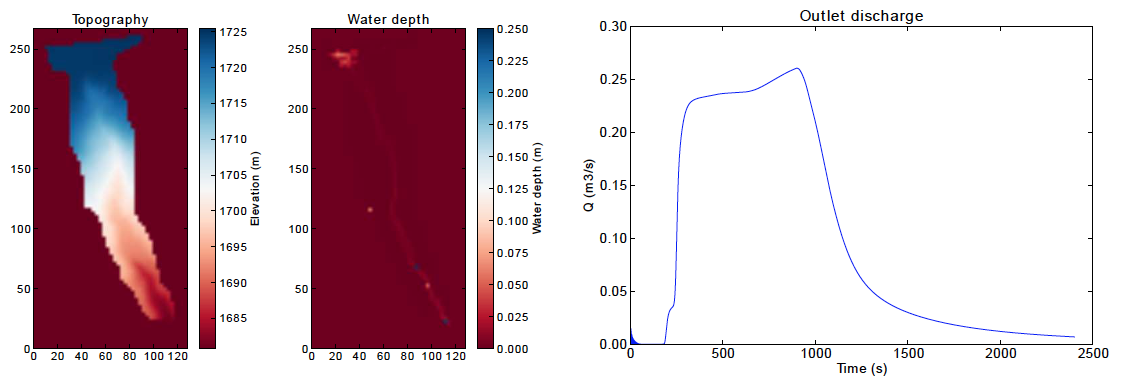
\includegraphics{overland_flow_dem.pdf}
    \caption{Output from a model of overland flow run on a DEM. Left: images showing topography, and water depth at end of run. Right: hydrograph at catchment outlet.}
   \label{olflowdem}
\end{figure}
%%%%%%%%%%%%%%%%%%%%%%%%%%%

\lstinputlisting[firstnumber=1,firstline=1,lastline=195]{overland_flow_with_model_grid_dem.py}

\subsection{Loading modules}

\lstinputlisting[firstnumber=11,firstline=11,lastline=15]{overland_flow_with_model_grid_dem.py}

In order to import the DEM, we will use Landlab's \code{read\_esri\_ascii} function, so we need to import this. We also need the Time module for timekeeping, OS for manipulating path names, Pylab for plotting, and Numpy for numerical operations. 

\subsection{User-defined variables}

\lstinputlisting[firstnumber=28,firstline=28,lastline=39]{overland_flow_with_model_grid_dem.py}

We will obtain topography from a 3-m resolution digital elevation model (DEM) of a small gully watershed in the West Bijou Creek drainage basin, east-central Colorado, USA. The drainage area of this catchment is about one hectare. The topography derives from airborne lidar data. The DEM is contained in an ArcInfo-format ascii file called {\em west\_bijou\_gully.asc}, located in the {\em ExampleDEM} folder.

In this example, we will allow flow through a single outlet cell, which we need to flag as a fixed-value boundary. We will also monitor discharge at the outlet. To accomplish these tasks, we need the row and column of the cell that will be used as the outlet and the cell next to it.

Our run will apply water as rainfall, with a rate given by \code{rainfall\_mmhr} and a duration given by \code{rain\_duration}. In fact, in this simple model, we won't allow any infiltration, so the rainfall rate is actually a runoff rate.

\subsection{Derived parameters}

\lstinputlisting[firstnumber=42,firstline=42,lastline=47]{overland_flow_with_model_grid_dem.py}

In this block of code, we convert the rainfall rate from millimeters per hour to meters per second. We also find the full path name of the input DEM by combining the pathname of the python code file (which is stored in \code{\_\_file\_\_}) with the specified DEM file name. We take advantage of the \code{dirname} and \code{join} functions in the OS module.

\subsection{Reading and initializing the DEM}

\lstinputlisting[firstnumber=49,firstline=49,lastline=56]{overland_flow_with_model_grid_dem.py}

ModelGrid's IO module allows us to read an ArcInfo ascii-format DEM with a call to the \code{read\_esri\_ascii} function. The function creates and returns a RasterModelGrid of the correct size and resolution, as well as a Numpy array of node elevation values. In this example, we know that the DEM contains elevations for a small watershed; nodes outside the watershed have a no-data value of zero. We don't want any flow to cross the watershed perimeter except at a single outlet cell. The call to the ModelGrid function \code{deactivate\_nodata\_nodes} accomplishes this by identifying all nodes for which the corresponding value in \code{z} equals the specified no-data value of zero.

\subsection{Setting up the watershed outlet}

\lstinputlisting[firstnumber=58,firstline=58,lastline=64]{overland_flow_with_model_grid_dem.py}

We will handle the outlet by keeping the water-surface slope the same as the bed-surface slope along the link that leads to the outlet boundary cell. To accomplish this, the first thing we need to do is find the ID of the outlet node and the interior node adjacent to it. We already know what the row and column numbers of these nodes are; to obtain the corresponding node ID, we use ModelGrid's \code{grid\_coords\_to\_node\_id} method. We then convert the outlet node to a fixed-value (i.e., open) boundary with the \code{set\_fixed\_value\_boundaries} method. (Note that in doing this, we've converted what was an interior node into a fixed boundary; had we converted a no-data node, we would end up with a waterfall at the outlet because the no-data nodes all have zero elevation, while the interior nodes all have elevations above 1600 m).

\subsection{Preparing to track discharge at the outlet}

\lstinputlisting[firstnumber=74,firstline=74,lastline=81]{overland_flow_with_model_grid_dem.py}

For this model, it would be nice to track discharge through time at the watershed outlet. To do this, we create two new lists: one for the time corresponding to each iteration, and one for the outlet discharge. Using lists will be slightly slower than using pre-defined Numpy arrays, but avoids forcing us to guess how many iterations there will be (recall that time-step size depends on the flow conditions in any given iteration). We append zeros to each list to represent the starting condition. To find out which active link represents the watershed outlet, we use ModelGrid's \code{get\_active\_link\_connecting\_node\_pair} method. This method takes a pair of node IDs as arguments. If the nodes are connected by an active link, it returns the ID of that active link; otherwise, it returns None.

\subsection{Main loop}

\lstinputlisting[firstnumber=119,firstline=119,lastline=124]{overland_flow_with_model_grid_dem.py}

Most of the main loop is identical to what we saw in Example 2, and here we will only list the parts that are new or different. One difference is that we now have a source term that represents rainfall and runoff. The code listed above sets the rainfall rate to zero when the elapsed time is greater than the rainfall duration. It also adds \code{rainfall\_rate} as a source term when computing $dh/dt$.

\lstinputlisting[firstnumber=135,firstline=135,lastline=137]{overland_flow_with_model_grid_dem.py}

After updating water depth values for the interior cells, we also need to update the water depth at the outlet boundary so that it matches the depth at the adjacent cell.

\lstinputlisting[firstnumber=142,firstline=142,lastline=144]{overland_flow_with_model_grid_dem.py}

The last few lines in the main loop keep track of discharge at the outlet by appending the current time and discharge to their respective lists.

\subsection{Plotting the result}

The plotting section is similar to what we saw in the previous two examples. One difference is that we now use two figures: one for the topography and water depth, and one for outlet discharge over time. We also use Pylab's sub-plot capability to place images of topography and water depth side by side.


%%%%%%%%%%%%%%%%%%%%%

\section{Using a Different Grid Type}

As noted earlier, ModelGrid provides several different types of grid. Available grids (as of this writing) are listed in Table~\ref{gridtypestable}.

\begin{table}[htbp]
   \centering
   \topcaption{List of available grid types} % requires the topcapt package
   \begin{tabular}{@{} lccl @{}} % Column formatting, @{} suppresses leading/trailing space
      \toprule
      
      %\cmidrule(r){1-2} % Partial rule. (r) trims the line a little bit on the right; (l) & (lr) also possible
      Grid type & Inherits from & Nodes & Cells \\
      \midrule
      RasterModelGrid  & ModelGrid & regular & square \\
      
      VoronoiDelaunayGrid & ModelGrid & Delaunay$^1$ & Voronoi$^2$ \\
      HexModelGrid & VoronoiDelaunayGrid & triagonal$^{1,3}$ & hexagonal$^4$ \\
      RadialModelGrid & VoronoiDelaunayGrid & concentric$^{1,5}$ & Voronoi$^2$ \\
      \bottomrule
      \multicolumn{4}{l}{$^1$ Nodes are connected by a Delaunay triangulation; user specifies node coordinates} \\
      \multicolumn{4}{l}{$^2$ Cells are Voronoi polygons} \\
      \multicolumn{4}{l}{$^3$ Nodes in regular triangular lattice with spacing $\delta$} \\
      \multicolumn{4}{l}{$^4$ Regular hexagons with side length $\delta/\sqrt{3}$ and area $\sqrt{3} \delta^2 / 2$} \\
      \multicolumn{4}{l}{$^5$ Points arranged in concentric circles with radial spacing $r$ and arc spacing $\approx r$} \\
   \end{tabular}
   %\caption{Remember, \emph{never} use vertical lines in tables.}
   \label{gridtypestable}
\end{table}

Suppose, for example, that we wanted to model a scenario in which the domain is a circular volcanic island. A radial, semi-structured arrangement of grid nodes might be a good solution. To run our diffusion model with this geometry, we only need to make some relatively simple changes. A radial model grid is defined by specifying a number of concentric ``shells'' of a given radial spacing, so we change lines 28--30 to:

\lstinputlisting[firstnumber=28,firstline=28,lastline=30]{diffusion_with_radial_model_grid.py}
Note that we have changed \code{dx} to \code{dr} on line 30. To create a RadialModelGrid instead of a RasterModelGrid, we simply replace the name of the object \code{RasterModelGrid} with \code{RadialModelGrid}:\footnote{These two types of grid are examples of the use of {\em inheritance}: each is a sub-class of \code{ModelGrid}, which means they both automatically contain all the methods and attributes of that base class.}

\lstinputlisting[firstnumber=39,firstline=39,lastline=39]{diffusion_with_radial_model_grid.py}
Finally, because our grid is now no longer a simple raster, we need to modify our plotting code. Here we'll replace the original plotting commands %(lines 74--94) 
with the following:

\lstinputlisting[firstnumber=75,firstline=75,lastline=94]{diffusion_with_radial_model_grid.py}
The result of our run is shown in Figure~\ref{radialdiffusion}.

%%%%%%%%%%% FIGURE %%%%%%%%%%%
 \begin{figure}[h!]
    \centering
    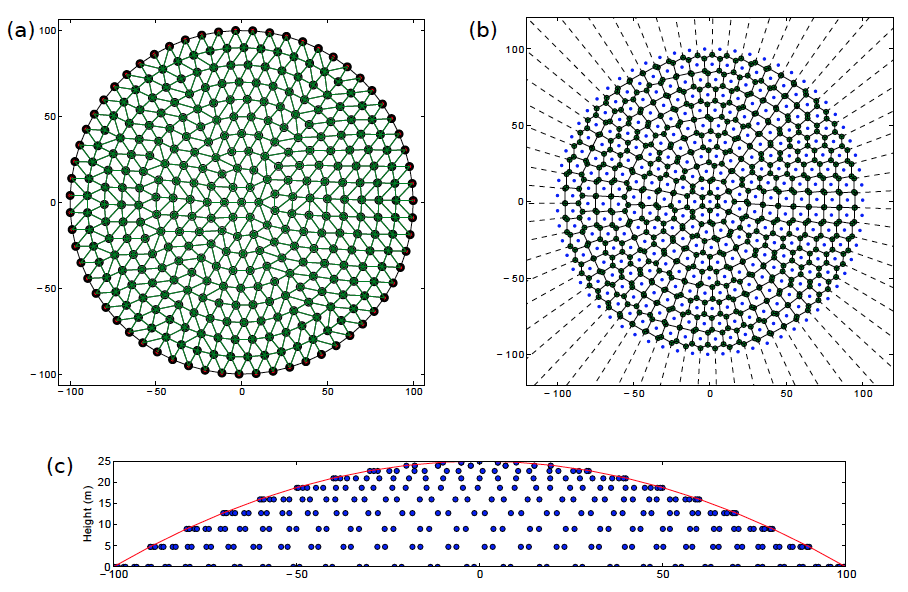
\includegraphics{radial_example.pdf}
    \caption{Diffusion model implemented with a radial model grid. (a) Nodes and links. Green nodes are active interior points, and red nodes are open boundaries. Active links in green; inactive links in black. Node gray shading is proportional to height. (b) Voronoi diagram, highlighting cells. Blue dots are nodes, and green circles are corners (cell vertices. Lines are faces (Voronoi polygon edges, sometimes called ``Voronoi ridges''). Dashed lines show orientation of undefined Voronoi edges. (c) Side view of model, showing nodes (blue dots) in comparison with analytical solution (red curve). All axes in meters.}
   \label{radialdiffusion}
\end{figure}
%%%%%%%%%%%%%%%%%%%%%%%%%%%



%%%%%%%%%%%%%%%%%%%%%

\section{Using ModelGrid with a Landlab Component}

[NOTE: THIS SECTION IS UNDER CONSTRUCTION]

So far, we've seen examples in which you use ModelGrid to create a new model from scratch. You can also use ModelGrid together with a pre-existing Landlab component to create a model. There are two ways to do this. The first is to create a Landlab Model, which is the recommended way to link together Landlab components because it provides helpful capabilities (such as easy file I/O and display handling, and compatibility with the CSDMS Framework). Instructions on how to create a Landlab Model are provided in {\em [NAME OF DOCUMENT]}. The second is simply to write a short Python program that instantiates one or more components, initializes them, and then uses a loop to call their \code{update} methods in turn. Here, we will illustrate this second method in order to give an introduction to how Landlab components work.

The listing below shows a version of the diffusion model in which we use a DiffusionComponent. In this case, the model parameters will be read from a formatted text file rather than being hard-coded (with one exception: we have hard-coded the name of the input file).

 \lstinputlisting[firstnumber=1,firstline=1,lastline=74]{example_diffusion_component_driver.py}

\subsection{Packages}

 \lstinputlisting[firstnumber=11,firstline=11,lastline=15]{example_diffusion_component_driver.py}

In addition to Numpy and Pylab, we will need ModelGrid, DiffusionComponent, and ModelParameterDictionary. The latter is a utility for reading model parameters and options from a formatted (ascii text) file.

\subsection{Display function}

[PROBABLY REPLACE THIS WITH INSTRUCTIONS ON USING MODELGRID BUILT-IN PLOTTING FUNCTION]

\subsection{Getting Input from a File}

\lstinputlisting[firstnumber=41,firstline=41,lastline=50]{example_diffusion_component_driver.py}

In this example, instead of putting the various input parameters directly in the code, we store them in a separate text file. This way, we can change the configuration and parameters of the model without altering the code itself. On line 46 we specify the name of the input file. The contents of this file are as follows:

\lstinputlisting{test_inputs_for_diffusion_model.txt}

The format of the file has two lines for each parameter. The first line contains a ``tag,'' which is a string of characters (by convention in ALL\_CAPS with underscores where needed) that denotes the name of the variable. The tag may be followed by a comment line. The next line contains the value of the parameter. Lines beginning with a hash mark (\#) are comments. Parameters can be listed in any order, though grouping related parameters makes it easier other human beings to read.

We open and read this file on line 49 by creating a ModelParameterDictionary and passing it the name of the file. A ModelParameterDictionary is a Python dictionary that contains the parameters listed in the file as key-value pairs. For example, after reading the file shown above, one of the dictionary entries in \code{mpd} will have NUM\_ROWS as the key and 20 as the value. 

On line 50, we retrieve the value for the parameter RUN\_DURATION, which is the duration of our model run in years. By passing the \code{ptype=float} argument, we guard errors in the input-file format; if the user, for example, wrote the string `thirty years', the code would produce an error because the value is not a floating-point number.

\subsection{Building the Grid and State Variable}

\lstinputlisting[firstnumber=52,firstline=52,lastline=56]{example_diffusion_component_driver.py}

In this example, we build and configure the grid in a single line of code, by calling ModelGrid's \code{create\_and\_initialize\_grid} function. This function takes a ModelParameterDictionary as an argument. It reads all the parameters necessary to determine the type of grid, the source (generated from scratch, read from a file, etc.), the boundary conditions, and other aspects. On line 56, we create our state variable, elevation (\code{z}), just as we did in previous examples.

\subsection{Creating and Initializing a Diffusion Component}

\lstinputlisting[firstnumber=58,firstline=58,lastline=60]{example_diffusion_component_driver.py}

All we need to do here is create a new instance of a diffusion component and then call its \code{initialize} method. When creating the component, we pass it the ModelGrid. This allows the component to create any internal variables it needs (such as sediment flux) that are tied to the grid. The \code{initialize} method takes a ModelParameterDictionary as an argument, and reads the necessary parameters. In our example input file above, there are two diffusion-related parameters, listed on lines 30--33: the creep coefficient (\code{DIFMOD\_KD}) and the effective uplift rate (\code{DIFMOD\_UPLIFT\_RATE}).

\subsection{Running the Diffusion Component}

\lstinputlisting[firstnumber=64,firstline=64,lastline=65]{example_diffusion_component_driver.py}

To run the diffusion component, we simply call its \code{run\_until} method, passing it the desired duration of the run and the elevation array. Recall that Numpy arrays (like other objects) are passed by reference, so that there is only one copy of \code{z}. The diffusion component will modify this copy, so that when the \code{run\_until} method finishes, we will have an altered (updated) elevation field.

\subsection{Cleaning Up}

\lstinputlisting[firstnumber=69,firstline=69,lastline=74]{example_diffusion_component_driver.py}

[SUBJECT TO CHANGE ONCE WE SORT OUT THE DISPLAY/WRITE]


\section{Terminology for grid elements}

[NOTE: THIS SHOULD BE WOVEN INTO TEXT IN THE INTRO, WHICH NEEDS TO BE UPDATED IN LIGHT OF REVISED TERMINOLOGY]

NODE: basic component of the grid. A node is a point with a unique $(x,y)$ location. Each node is connected to one or more neighboring nodes by a LINK. The $i^{th}$ node is denoted $N_i$, and its location is $(x_i, y_i)$. 

CELL: a cell is a polygon that contains one (and only one) node. Every cell contains an associated node, but nodes on the perimeter of a grid do not have cells.

LINK: a link is a line segment that connects two NODES. Each link has a direction as well as a position in space. A link


\section{Getting information about the grid and its elements}

NODE location: grid.node\_x, grid.node\_y






%%%%%%%%%%%%%%%%%%%%%
\newpage
\bibliography{/Users/gtucker/Documents/Literature/gt_library.bib}
\bibliographystyle{/Users/gtucker/Documents/Literature/agufull08}



\end{document}